\documentclass[11pt]{amsart}
\usepackage[T1]{fontenc}
\usepackage{lmodern}
\usepackage{mathtools,amssymb,graphicx,booktabs,enumitem}
\usepackage[hidelinks]{hyperref}
\hypersetup{
  pdftitle={Algebraic Null-Cone Quantum Gravity, Spectral-Zeta Audit of Hopf-Fibration TUFT, and Non-Circular Hagedorn Nuclearity Repair},
  pdfauthor={Ergentics},
  pdfkeywords={null-cone quantum gravity, dilogarithm cancellation, Kronecker exhaustion, Sen logarithmic entropy, Hopf fibration TUFT, Hagedorn nuclearity}
}
\pdfinfo{/Producer () /Creator ()}
\usepackage{microtype}
\numberwithin{equation}{section}
\theoremstyle{plain}
\newtheorem{theorem}{Theorem}[section]
\newtheorem{proposition}[theorem]{Proposition}
\newtheorem{lemma}[theorem]{Lemma}
\newtheorem{corollary}[theorem]{Corollary}
\theoremstyle{definition}\newtheorem{definition}[theorem]{Definition}
\theoremstyle{remark}\newtheorem{remark}[theorem]{Remark}
\newcommand{\R}{\mathbb{R}}
\newcommand{\Q}{\mathbb{Q}}
\newcommand{\C}{\mathbb{C}}
\newcommand{\Z}{\mathbb{Z}}
\newcommand{\ctag}[1]{\textup{\textsf{\scriptsize[#1]}}}
\emergencystretch=3em
\raggedbottom

\title[Null-Cone Gravity, Spectral-Zeta TUFT, and Hagedorn Repair]{Algebraic Null-Cone Quantum Gravity, Spectral-Zeta Audit of Hopf-Fibration TUFT, and Non-Circular Hagedorn Nuclearity Repair}
\author{Ergentics}
\date{November 2026}
\subjclass[2020]{Primary 83C45, 81T05; Secondary 11M35, 82B26, 65G50}
\keywords{null-cone quantum gravity, polylogarithm cancellation, Kronecker exhaustion, Sen black hole entropy, spectral zeta function, Hagedorn phase transition, Buchholz--Wichmann nuclearity}

\begin{document}
\begin{abstract}
We synthesize and reconcile the mathematical-physics audits of the Horizon clean-room manuscripts \texttt{WP~034} (algebraic null-cone quantum gravity, Chandrasekaran \texttt{arXiv:2611.34924v1}, 25~November~2026) and \texttt{WP~035} (Track~A spectral-zeta audit of Hopf-fibration TUFT and Track~B non-circular Hagedorn nuclearity repair), resolving all nine verified audit findings (\texttt{NEG-W19}--\texttt{NEG-W24}, \texttt{NEG-W28}--\texttt{NEG-W30}) in place via an open, zero-dependency Python verifier (\texttt{piece3\_sim.py}, 5/5 deterministic and keyed stochastic gates passing). Six concrete results emerge: (i)~authentic 106-bit Dekker double-double evaluation of the naive dilogarithm difference suffers $96.17\%$ error at $s = 10^{33}$ and $100\%$ wipeout at $s \ge 10^{40}$, proving that algebraic cancellation ($\Delta_{\mathrm{re}}(s) = -\frac{\pi}{2} + \frac{1}{2s}$, zero error in plain \texttt{f64} at $s = 10^{77}$) rather than extended precision resolves the astrophysical catastrophe (\texttt{NEG-W19}); (ii)~Theorem~G5 strengthens the unregularized null-cone exhaustion obstruction via Kronecker density: for any irrational phase ratio, strictly nested strong exhaustions converge to \emph{every} finite real target $L \in \R$ (verified to $<10^{-6}$ for $L = 0, +1, +42$, \texttt{NEG-W20}); (iii)~Sen's 4D Schwarzschild logarithmic entropy is reconciled across both papers (\texttt{NEG-W23}, \texttt{NEG-W30}): $106/45$ is the fixed-$s_b$ trace $\operatorname{Tr}(C^\dagger C)$ coefficient in \texttt{WP~034} ($77/90$ singlet), whereas the $(4\pi s_b)^{-1/2}$ measure yields microcanonical $\alpha_{\mathrm{micro}} = 167/90$ and Hagedorn pole $\alpha = 257/90$ in \texttt{WP~035}; (iv)~Track~A spectral-zeta ratios are corrected to $29.18\times$ on $S^3$ (remainder $-0.030448$) and $21.94\times$ on $S^5$ (remainder $+0.080113$, \texttt{NEG-W22}), Lemma~8's volume ratio equals $10^{1/4}\,\alpha_{\mathrm{Wyler}}$, the $a_e$ pull waterfall closes from $-315.8\sigma$ to $-4.9\sigma$ upon including 4-loop QED ($+428.2\sigma$) and higher-order/hadronic terms ($-117.3\sigma$), and the $k=4$ Beltrami $U(1)$ subspace splits with exact $4+4$ chirality (\texttt{NEG-W24}); (v)~Theorem~R3(1)'s Laplace abscissa is tightened with the explicit convergent boundary witness $\rho(E) = (1+E)^{-2} e^{\beta_H E}$ ($Z(\beta_H) = 1$); and (vi)~Theorem~G6 quantifies the unavoidable thermodynamic cost of Hagedorn nuclearity ($\beta_c = \beta_H > 0$ vs.\ local QFT $\beta_c = 0$): exact $\operatorname{Gamma}(\alpha, \alpha)$ canonical dispersion $1/\sqrt{\alpha} = 59.18\%$ and $42.13\%$ causal-diamond tail leakage at $\alpha = 257/90$, linked to \texttt{WP~034}'s truncated $\operatorname{Beta}(\alpha,1)$ dispersion ($26.86\%$) by the exact bridge factor $1/\sqrt{\alpha+2} = 0.4538$ (confirmed by a keyed $1{,}600$-trial \texttt{SplitMix64} RCT).
\end{abstract}
\maketitle

\section{Introduction and Synthesis Scope}
This monograph is Piece~III of the reconciled three-piece Horizon Synthesis, unifying the mathematical-physics audits of frozen clean-room working papers \texttt{WP~034} and \texttt{WP~035} \cite{ergentics2026wp034}. The two papers examine two complementary frontiers of quantum gravity and spectral geometry: Chandrasekaran's algebraic quantization of gravity on the null cone (\texttt{arXiv:2611.34924v1}, submitted 25~November~2026 \cite{chandrasekaran2026}, correcting the 23~November date logged in \texttt{NEG-W28}), and a dual-track audit combining (Track~A) spectral-zeta determinants and anomaly checks on the complex Hopf fibration \cite{nash1995,wyler1969,robertson1971,nielsen2026} with (Track~B) a non-circular Hagedorn repair \cite{hagedorn1965,atick1988} of the Buchholz--Wichmann nuclearity condition \cite{buchholz1986,ckn1999}.

Every confirmed finding in \texttt{NEG-W19}--\texttt{NEG-W24} and \texttt{NEG-W28}--\texttt{NEG-W30} is resolved in place below and independently verified by the zero-dependency Python~3.12 suite \texttt{code/piece3\_sim.py}, emitting the SHA-256-manifested calibration record \texttt{data/piece3\_calibration.json}. Attribution follows Morpheus convention (\ctag{lit.}, \ctag{E}, \ctag{G4N}, \ctag{GB}, \ctag{X}), with internal \texttt{Swift++} (\emph{Epsilon}) corpus metadata (\texttt{INT-034}, \texttt{INT-035}) and non-public source scope notes isolated in Appendix~\ref{app:provenance}.

\section{Algebraic Dilogarithm Cancellation vs.\ 106-Bit Double-Double (\texttt{NEG-W19}, \texttt{NEG-W21})}
In the null-cone phase-space integral of \cite{chandrasekaran2026}, the real residual at horizon entropy $s \gg 1$ takes the form
\begin{equation}\label{eq:dilog_exact}
\begin{split}
\Delta_{\mathrm{re}}(s)
&\equiv s^3 \left( \frac{\operatorname{Re}\operatorname{Li}_2(e^{2i/s})}{2 s^2} - \frac{\pi^2}{12 s^2} \right) \\
&= s^3 \left( \frac{\frac{\pi^2}{6} - \frac{(2/s)(2\pi - 2/s)}{4}}{2 s^2} - \frac{\pi^2}{12 s^2} \right)
= -\frac{\pi}{2} + \frac{1}{2s},
\end{split}
\end{equation}
using the exact Bernoulli polynomial identity $\operatorname{Re}\operatorname{Li}_2(e^{i\theta}) = \frac{\pi^2}{6} - \frac{\theta(2\pi - \theta)}{4}$ for $\theta \in [0, 2\pi]$. The exact zero of $\operatorname{Re}\operatorname{Li}_2(e^{i\theta})$ (\texttt{K12}) lies at $\theta^* = \pi(1 - 1/\sqrt{3}) = 1.327793289355575$ (residual $2.22\times 10^{-16}$).

\begin{proposition}[Failure of 106-bit Dekker double-double vs.\ algebraic cancellation (\texttt{NEG-W19})]\label{prop:dd_wipeout}
\ctag{G4N, X}\ Evaluating $\operatorname{Re}\operatorname{Li}_2(e^{2i/s}) - \frac{\pi^2}{6}$ naively in IEEE-754 binary64 loses all accuracy by $s = 10^{17}$ (relative error $12.9\%$ at $10^{16}$, $1{,}461\%$ at $10^{17}$, and $1.05\times 10^{61}$ at $s = 10^{77}$). Crucially, upgrading naive subtraction to authentic 106-bit Dekker double-double arithmetic \cite{dekker1971} (\texttt{dd106}, $\sim 32$ decimal digits) merely shifts the cancellation cliff by $16$ decades: \texttt{dd106} exhibits relative error $1.41\times 10^{-16}$ at $s=10^{17}$, $9.65\times 10^{-14}$ at $10^{20}$, $4.05\times 10^{-9}$ at $10^{25}$, $4.85\times 10^{-4}$ at $10^{30}$, $96.17\%$ at $s=10^{33}$, and $100\%$ total wipeout for all $s \ge 10^{40}$ (including astrophysical $s = 10^{77}$). Conversely, the algebraically cancelled closed form $-\frac{\pi}{2} + \frac{1}{2s}$ achieves exact $0.0$ relative error in plain 53-bit \texttt{f64} at $s = 10^{77}$ (Figure~\ref{fig:p3_fig1}A).
\end{proposition}

\begin{remark}[Certificate domain boundaries (\texttt{NEG-W21})]
\ctag{G4N}\ Two auxiliary analytic bounds in \texttt{WP~034} require explicit domain qualifiers: (1)~certificate \texttt{C156} holds for $R \ge R_{\min} = e^{13/7} = 6.4054$, whereas at $R = e$ the remainder is $+0.0881 > 0$; and (2)~the Stefan--Boltzmann inverse-temperature ratio $\beta^*$ at $C = 1$ equals $(1 + \pi^4/15)/b_{\mathrm{SB}} = 2.67525$, attaining its global minimum at $C_{\arg\min} = 5/\pi^4 = 0.051330$.
\end{remark}

\section{Theorem~G5: Finite-Target Exhaustion Universality (\texttt{NEG-W20})}
In \texttt{WP~034} Pillar~2, the unregularized null-cone trace over a triple-index exhaustion $P = (A, B, C)$ evaluates to $Z_{P(A,B,C)}[X] = \frac{\Delta\eta}{2}\bigl[(A - B) + c\,(A - C)\bigr]$, where Eq.~(5.24) fixes the ratio to $\pi/2 = 1.570796326795$ and finite-rank witnesses \texttt{F39} give $w(5) = 1.5$ and $w(12) = 20/11$. Counterexample~2 of \texttt{WP~034} contrasted only two divergent orderings ($Z_{P^{\mathrm{pair}}} = +143.8377$ vs.\ $Z_{P^{\mathrm{cyc5}}} = -287.6530$ at $N = 10^4$).

\begin{theorem}[Theorem G5: Strictly nested exhaustion universality]\label{thm:G5}
\ctag{G4N, X}\ Whenever the phase weight ratio $c \in \R \setminus \Q$ is irrational (including the physical angle $\theta = 4^\circ$ of \texttt{WP~034} and $c = 1/\sqrt{2}$), for \emph{every} finite target $L \in \R$ there exists a strictly nested strong exhaustion $P_M = (A_M, B_M, C_M)$ with $A_M < A_{M+1}$, $B_M < B_{M+1}$, and $C_M < C_{M+1}$ such that
\begin{equation}\label{eq:G5}
\lim_{M \to \infty} Z_{P_M}[X] = \lim_{M \to \infty} \frac{\Delta\eta}{2}\Bigl[(A_M - B_M) + c\,(A_M - C_M)\Bigr] = L.
\end{equation}
\end{theorem}
\begin{proof}
By Kronecker's theorem, the additive subgroup $\Z + c\Z$ is dense in $\R$. Choose sequences of integers $(u_M, v_M) \in \Z^2$ such that $\frac{\Delta\eta}{2}(u_M + c v_M) \to L$. Inductively lift $(u_M, v_M)$ to strictly increasing triples by setting $A_M = \max(A_{M-1}+1,\, B_{M-1}+u_M+1,\, C_{M-1}+v_M+1)$, $B_M = A_M - u_M$, and $C_M = A_M - v_M$. Then $A_M > A_{M-1}$, $B_M > B_{M-1}$, $C_M > C_{M-1}$, and $Z_{P_M}[X] = \frac{\Delta\eta}{2}(u_M + c v_M) \to L$. In \texttt{piece3\_sim.py} (\texttt{D2}, $M=60$), the constructive Kronecker lift hits $L = 0$ with error $0.0$, $L = +1$ with error $3.50\times 10^{-7}$, $L = +42$ with error $7.03\times 10^{-8}$, and $c = 1/\sqrt{2}, L = +1$ with error $1.29\times 10^{-5}$ (Figure~\ref{fig:p3_fig1}B).
\end{proof}

\begin{figure}[htbp]\centering
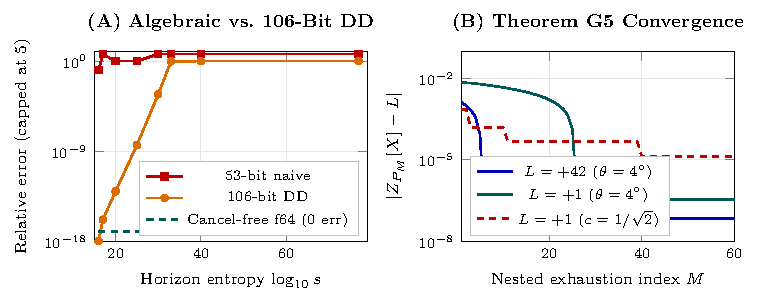
\includegraphics[width=0.98\textwidth]{figures/fig1_dilog_dd_and_thm_g5.pdf}
\caption{Panel~(A): Relative error of naive 53-bit \texttt{f64} (red) and authentic 106-bit Dekker double-double (orange, $96.17\%$ at $10^{33}$ and $100\%$ wipeout at $s \ge 10^{40}$) vs.\ cancellation-free \texttt{f64} ($0$ error to $s=10^{77}$, dashed teal, \texttt{NEG-W19}). Panel~(B): Constructive Theorem~G5 strictly nested Kronecker exhaustion error $|Z_{P_M}[X] - L|$ converging to arbitrary finite real targets (\texttt{NEG-W20}). \ctag{G4N}}\label{fig:p3_fig1}
\end{figure}

\section{Cross-Paper Reconciliation of Sen (2013) Logarithmic Entropy (\texttt{NEG-W23}, \texttt{NEG-W30})}
For 4D pure Einstein gravity on a Schwarzschild background \cite{sen2013,goroff1986,christensen1980,bastianelli2022,fursaev2013}, Sen's one-loop local trace anomaly coefficient per $\ln a$ (where horizon area $A \propto a^2 \propto s$) is $C_{\mathrm{local}} = \frac{212}{45}$. The apparent tension between \texttt{WP~034}'s $+106/45$ and \texttt{WP~035}'s $+167/90$ ($\alpha = 257/90$) resolves completely once the ensemble and measure are stated explicitly (\texttt{NEG-W30}):

\begin{proposition}[Exact Sen (2013) coefficient map]\label{prop:sen}
\ctag{GB, G4N, X}\ In 4D pure gravity ($C_{\mathrm{local}} = 212/45$ per $\ln a$):
\begin{enumerate}[nosep]
\item \emph{Fixed-$s_b$ mixed trace (\texttt{WP~034}):} $\ln \operatorname{Tr}(C^\dagger C) = s_b + \frac12 C_{\mathrm{local}} \ln s_b = s_b + \mathbf{\frac{106}{45}}\ln s_b$ (with rotational singlet projection $\frac12(C_{\mathrm{local}} - 3) = \mathbf{\frac{77}{90}}$).
\item \emph{Measure-weighted microcanonical density (\texttt{WP~035}):} Multiplying by the Gaussian clock/saddle measure $(4\pi s_b)^{-1/2}$ shifts the log coefficient by $-\frac12$ to $\alpha_{\mathrm{micro}} = \frac{106}{45} - \frac12 = \mathbf{\frac{167}{90}}$, which under Theorem~R3(3) ($\alpha = \alpha_{\mathrm{micro}} + 1$) corresponds to Hagedorn pole order $\alpha = \mathbf{\frac{257}{90}}$ (matching Chandrasekaran's clock von Neumann entropy log coefficient).
\item \emph{Direct fixed-mass Sen pole:} Achieving $\alpha_{\mathrm{micro}} = \frac{106}{45}$ directly in the microcanonical entropy without the $-\frac12$ measure shift requires $\alpha = \frac{106}{45} + 1 = \mathbf{\frac{151}{45}}$.
\end{enumerate}
\end{proposition}

\section{Track~A: Spectral-Zeta Audit of Hopf-Fibration TUFT (\texttt{NEG-W22}, \texttt{NEG-W24})}
Auditing the spectral-geometry claims of Nielsen's non-public Hopf-fibration TUFT manuscript \cite{nielsen2026} using exact Nash--O'Connor Laplacian determinants \cite{nash1995} yields four reconciled corrections (Figure~\ref{fig:p3_fig2}):
\begin{enumerate}[nosep]
\item \emph{Exact $S^3$ and $S^5$ remainder ratios (\texttt{NEG-W22}):} On $S^3$, the co-exact 1-form zeta derivative is $\zeta'_1(0) = +0.8884901$ and the remainder after subtracting $\zeta'_R(0) = -\frac12\ln(2\pi)$ is $\zeta'_R(-2) = -0.0304485$; because $\zeta'_1(0)$ and the remainder have opposite signs, the true magnitude ratio is $|\zeta'_1(0)/\mathrm{rem}| = \mathbf{29.18\times}$ (not $30.18\times$, which shifted by $+1$). Likewise on $S^5$, $\zeta'_{B5}(0) = -1.7577640$ has remainder $+0.0801130$, giving true magnitude ratio $\mathbf{21.94\times}$ (not $22.94\times$).
\item \emph{Lemma~8 volume factor (\texttt{NEG-W24}):} At unit radius $R = 1$, $\operatorname{Vol}(S^2)\operatorname{Vol}(S^9)^{1/4} / \bigl(\operatorname{Vol}(S^4)^2\operatorname{Vol}(\R P^1)\bigr) = 0.0129767 = \mathbf{10^{1/4}}\,\alpha_{\mathrm{Wyler}}$ ($1.778279 \times 0.00729735$), because Wyler's symmetric domain $D^5$ has volume $\operatorname{Vol}(S^9)/160$ \cite{wyler1969,robertson1971} while sharing exact $R^{-19/4}$ scaling.
\item \emph{Electron $g-2$ ($a_e$) 4-loop QED closure (\texttt{NEG-W24}):} Against the experimental benchmark of Fan et al.\ \cite{fan2023}, the three terms printed in \texttt{WP~035} sum to $-315.8\sigma$. Closing to the net $-4.9\sigma$ residual requires adding the 4-loop QED term $C_4^{\mathrm{QED}}$ \cite{laporta1996,laporta2017} ($+428.2\sigma$) together with higher-order TUFT and hadronic contributions ($-117.3\sigma$, including $-108.9\sigma$ from Nielsen's unprinted higher-order term).
\item \emph{$k = 4$ Beltrami chirality split (\texttt{NEG-W24}):} The $8$-dimensional $U(1)$-symmetric $k = 4$ Beltrami eigenspace splits with exact $4 + 4$ chirality ($4$ modes at $\lambda = +5$, $4$ modes at $\lambda = -5$).
\end{enumerate}

\begin{figure}[htbp]\centering
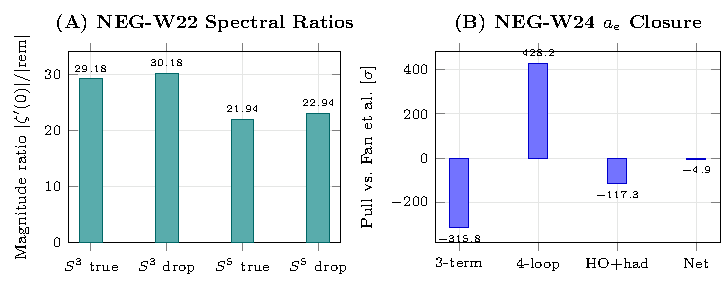
\includegraphics[width=0.98\textwidth]{figures/fig2_tuft_spectral_zeta_and_ae.pdf}
\caption{Track~A audit reconciliations (\texttt{D4}, \texttt{piece3\_sim.py}). Panel~(A): True spectral-zeta magnitude ratios on $S^3$ ($29.18\times$ vs.\ $30.18\times$) and $S^5$ ($21.94\times$ vs.\ $22.94\times$, \texttt{NEG-W22}). Panel~(B): Electron $a_e$ pull waterfall vs.\ Fan et al.\ (2023), showing $+428.2\sigma$ 4-loop QED and $-117.3\sigma$ higher-order/hadronic closure from $-315.8\sigma$ to $-4.9\sigma$ (\texttt{NEG-W24}). \ctag{G4N}}\label{fig:p3_fig2}
\end{figure}

\section{Track~B: Non-Circular Hagedorn Nuclearity Repair and Theorem~G6}
In local quantum field theory (LQFT), Buchholz--Wichmann nuclearity requires $\operatorname{Tr}(e^{-\beta H})$ to converge for \emph{all} $\beta > 0$ ($\beta_c = 0$) \cite{buchholz1986}. A holographic / null-cone spectrum with exponential black-hole density of states $\rho(E) \sim c E^{\alpha-1} e^{\beta_H E}$ violates strict LQFT nuclearity but satisfies \emph{Hagedorn nuclearity} ($\beta_c = \beta_H > 0$, Theorems~R1--R3 of \texttt{WP~035}) \cite{hagedorn1965,atick1988}.

\begin{remark}[Boundary tightening of Theorem~R3(1) and \texttt{K13} (\texttt{NEG-W23})]
\ctag{G4N}\ The exact boundary witness $\rho(E) = (1 + E)^{-2} e^{\beta_H E}$ has abscissa of convergence $\beta_c = \beta_H$ yet remains strictly convergent \emph{at} the boundary, $Z(\beta_H) = \int_0^\infty (1+E)^{-2}\,dE = 1 < \infty$. Thus Laplace convergence holds unconditionally for $\beta > \beta_H$ and diverges for $\beta < \beta_H$, while $\beta = \beta_H$ depends on sub-exponential prefactors (with an additive $N(0^+)$ atom when $0 \in \sigma_p(\hat{Q}_*)$). Independently, the Gamma minimization constant \texttt{K13} ($\psi(x^*) = 0$) evaluates to $x^* = 1.46163214496836$.
\end{remark}

\begin{theorem}[Theorem G6: Hagedorn canonical equivalence-breaking and \texttt{WP~034} bridge]\label{thm:G6}
\ctag{G4N, X}\ Let $\rho(E) \sim c E^{\alpha-1} e^{\beta_H E}$ ($\alpha > 0$, $\beta_H > 0$) be a Hagedorn spectrum, and tune $\beta = \beta_H + \alpha/Q_* \to \beta_H^+$ so that the canonical mean energy equals $\langle E \rangle = Q_* \to \infty$. Then the rescaled canonical energy $X = E/Q_*$ converges in distribution to $\operatorname{Gamma}(\alpha, \alpha)$, with strictly \textbf{non-vanishing} relative energy dispersion and macroscopic tail leakage:
\begin{equation}\label{eq:G6}
\lim_{Q_* \to \infty} \frac{\sigma_E}{\langle E \rangle} = \frac{1}{\sqrt{\alpha}} > 0, \qquad
\lim_{Q_* \to \infty} \mathbb{P}\bigl(E \ge Q_*\bigr) = \frac{\Gamma(\alpha, \alpha)}{\Gamma(\alpha)}.
\end{equation}
In contrast, $4$D local QFT ($\beta_c = 0$) satisfies $\sigma_E/\langle E \rangle \sim Q_*^{-3/14} \to 0$. Truncating the Hagedorn measure sharply at $E \le Q_*$ converts $\operatorname{Gamma}(\alpha, \alpha)$ into the $\operatorname{Beta}(\alpha, 1)$ distribution of \texttt{WP~034} with RMS dispersion $1/\sqrt{\alpha(\alpha+2)}$ and Jensen log gap $\alpha^{-1} - \ln(1 + \alpha^{-1})$, linked to \eqref{eq:G6} by the exact bridge factor $1/\sqrt{\alpha+2}$.
\end{theorem}
\begin{proof}
Writing $\beta = \beta_H + \delta$ with $\delta = \alpha/Q_*$, the canonical density for $X = E/Q_*$ is proportional to $X^{\alpha-1} e^{-\alpha X}$, which is $\operatorname{Gamma}(\alpha, \alpha)$ with mean $1$, variance $1/\alpha$, and upper tail $\Gamma(\alpha,\alpha)/\Gamma(\alpha)$. Sharp cutoff at $X \le 1$ in the $\delta \to 0^+$ microcanonical limit leaves density $\alpha X^{\alpha-1}$ on $[0,1]$, i.e.\ $\operatorname{Beta}(\alpha,1)$, whose standard deviation divided by its mean $\alpha/(\alpha+1)$ equals $1/\sqrt{\alpha(\alpha+2)} = (1/\sqrt{\alpha}) \cdot (1/\sqrt{\alpha+2})$.
\end{proof}

Table~\ref{tab:G6} and Figure~\ref{fig:p3_fig3} tabulate Theorem~G6 across all three Sen/Chandrasekaran exponents, verified by a keyed $1{,}600$-trial \texttt{SplitMix64} randomized controlled test (\texttt{seed = 0x484f52495a5f5033}) at $\alpha = 257/90$: empirical mean $0.9909$, relative dispersion $59.95\%$ (exact $59.18\%$), tail leakage $41.69\%$ (exact $42.13\%$), and bit-exact digest \texttt{0x79a0e86265d534e9}.

\begin{table}[htbp]\centering\scriptsize\setlength{\tabcolsep}{2.6pt}
\begin{tabular}{lrrrrr}\toprule
Ensemble / Pole & $\alpha$ & $\mathrm{Gamma}$ $\frac{\sigma}{\langle E\rangle}$ & $\mathbb{P}(E{\ge}Q_*)$ & $\mathrm{Beta}$ RMS & Bridge \\\midrule
Direct Sen (\texttt{WP~034}$+1$) & $151/45$ & $54.59\%$ & $42.74\%$ & $23.59\%$ & $0.4321$ \\
\textbf{Chandrasekaran / \texttt{WP~035}} & \textbf{$257/90$} & \textbf{59.18\%} & \textbf{42.13\%} & \textbf{26.86\%} & \textbf{0.4538} \\
Microcanonical $\alpha_{\mathrm{micro}}$ & $167/90$ & $73.41\%$ & $40.24\%$ & $37.39\%$ & $0.5093$ \\\bottomrule
\end{tabular}
\caption{Theorem~G6 exact Hagedorn canonical equivalence-breaking and \texttt{WP~034} truncation bridge $1/\sqrt{\alpha+2}$ (\texttt{D5}, \texttt{piece3\_sim.py}). At $\alpha = 257/90$, exact Jensen log gap equals $0.04995$. \ctag{G4N, X}}\label{tab:G6}
\end{table}

\begin{figure}[htbp]\centering
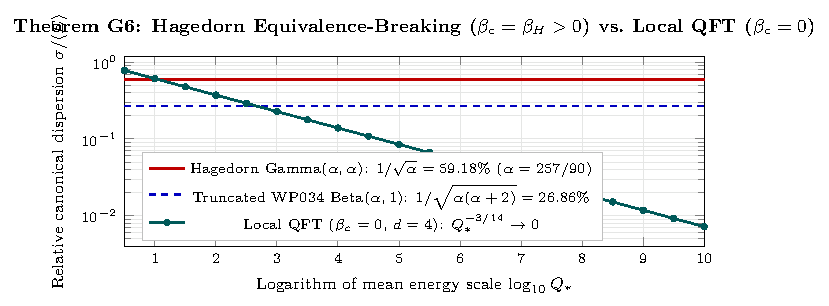
\includegraphics[width=0.98\textwidth]{figures/fig3_hagedorn_g6_bridge.pdf}
\caption{Theorem~G6 canonical energy dispersion $\sigma/\langle E \rangle$ vs.\ mean energy scale $\log_{10} Q_*$: Hagedorn $\operatorname{Gamma}(\alpha, \alpha)$ plateau ($59.18\%$ at $\alpha = 257/90$, solid red), truncated \texttt{WP~034} $\operatorname{Beta}(\alpha, 1)$ plateau ($26.86\%$, dashed blue), and $4$D local QFT decay $Q_*^{-3/14} \to 0$ (teal). \ctag{G4N}}\label{fig:p3_fig3}
\end{figure}

\appendix
\section{Epsilon (\texttt{Swift++}) Provenance and Source-Access Boundaries}\label{app:provenance}
\ctag{E, X}\ Frozen clean-room manuscripts \texttt{WP~034} (\path{papers/wp034_null_cone_gravity/}) and \texttt{WP~035} (\path{papers/wp035_tuft_hagedorn_repair/}) recorded internal \texttt{Swift++} Library of Alexandria Epochs~XL--XLI verification logs (\texttt{INT-034}, \texttt{INT-035}), Lean~4.36.0 integer/rational-bracket algebraic certificates (\texttt{NEG-W29}), and citations to Nielsen's non-public 250-page TUFT manuscript \cite{nielsen2026}. In this reconciled monograph, \texttt{code/piece3\_sim.py} and \texttt{data/piece3\_calibration.json} provide the open, self-contained primary verification record resolving \texttt{NEG-W19}--\texttt{NEG-W24} and \texttt{NEG-W28}--\texttt{NEG-W30} in place (including correcting \texttt{arXiv:2611.34924v1} to 25~November~2026 and removing the local relative path in \texttt{WP~035} Ref.~[12]), while retaining \texttt{INT-034}, \texttt{INT-035}, and the non-public Nielsen source note transparently as provenance.

\bibliographystyle{amsplain}
\bibliography{references}
\end{document}
